% !TEX program = xelatex
\documentclass[12pt, a4paper]{article}

% ---- Chinese support ----
\usepackage[UTF8, zihao=-4]{ctex}
\setCJKmainfont{SimSun}[BoldFont=SimHei, ItalicFont=KaiTi]
\setCJKsansfont{SimHei}
\setCJKmonofont{FangSong}

% ---- Page layout ----
\usepackage[top=2.5cm, bottom=2.5cm, left=3cm, right=3cm]{geometry}
\usepackage{setspace}
\onehalfspacing

% ---- Math ----
\usepackage{amsmath, amssymb, amsthm}
\usepackage{bm}

% ---- Tables ----
\usepackage{booktabs}
\usepackage{array}
\usepackage{multirow}
\usepackage{longtable}
\usepackage{tabularx}
\usepackage{threeparttable}

% ---- Figures ----
\usepackage{graphicx}
\usepackage{caption}
\usepackage{subcaption}
\usepackage{float}

% ---- Typography ----
\usepackage{microtype}
\usepackage{indentfirst}
\setlength{\parindent}{2em}
\usepackage{enumitem}

% ---- Colors & Links ----
\usepackage[dvipsnames]{xcolor}
\usepackage[colorlinks=true, linkcolor=NavyBlue, citecolor=NavyBlue,
            urlcolor=NavyBlue, bookmarks=true]{hyperref}

% ---- Header / Footer ----
\usepackage{fancyhdr}
\pagestyle{fancy}
\fancyhf{}
\fancyhead[L]{\small\kaishu 宽带基础设施与县级制造业TFP}
\fancyhead[R]{\small\thepage}
\renewcommand{\headrulewidth}{0.4pt}

% ---- Section formatting ----
\usepackage{titlesec}
\titleformat{\section}{\large\bfseries\heiti}{\thesection}{1em}{}
\titleformat{\subsection}{\normalsize\bfseries\heiti}{\thesubsection}{1em}{}
\titleformat{\subsubsection}{\normalsize\heiti}{\thesubsubsection}{1em}{}

% ---- Bibliography ----
\usepackage[authoryear, round]{natbib}
\bibliographystyle{plainnat}

% ---- Abstract environment ----
\usepackage{abstract}
\renewcommand{\abstractnamefont}{\large\bfseries\heiti}
\setlength{\absleftindent}{1.5em}
\setlength{\absrightindent}{1.5em}

% ---- Footnotes ----
\usepackage{footmisc}

% ---- Misc ----
\usepackage{xspace}
\newcommand{\ie}{\textit{i.e.}\xspace}
\newcommand{\eg}{\textit{e.g.}\xspace}

% ============================================================
\begin{document}
% ============================================================

% ---- Title ----
\begin{titlepage}
\centering
\vspace*{2cm}
{\LARGE\heiti 宽带基础设施与县级制造业全要素生产率\par}
\vspace{0.5em}
{\large\heiti ——来自"宽带中国"准自然实验的因果证据\par}
\vspace{2cm}
{\large 作者预留\par}
\vspace{0.5em}
{\normalsize 单位预留 \quad \textit{zongrong@tamu.edu}\par}
\vspace{2cm}
{\normalsize \today\par}
\vspace{3cm}
\begin{abstract}
\noindent
本文利用"宽带中国"示范城市分批次遴选所形成的准自然实验，采用
Callaway \& Sant'Anna（2021）CS-DiD估计量，识别宽带基础设施建设对辖区
县级制造业全要素生产率（TFP）的因果效应。基于2010—2018年300个县级单元
的平衡面板数据（$N=2700$），本文发现：第一，宽带中国政策使县级制造业
TFP平均提升0.1117个对数点（SE$=0.0062$，$p<0.01$），相当于样本均值的4.3\%；
效应于政策实施当年即显现，并在此后四年持续稳定，无衰减迹象。第二，机制
检验表明，政策通过专利创新渠道传导约5.7\%的TFP效应，但要素配置效率提升
是更主导的传导机制。第三，效应在空间上高度不均：东部县效应（$\hat\beta=0.1403$）
约为西部县（$\hat\beta=0.0836$）的1.67倍；大规模县域效应（$\hat\beta=0.1279$）
较小县高46\%，显示出网络外部性与互补资产的空间集聚特征。上述结论在
5项稳健性检验下保持不变。本文为宽带基础设施投资提供了县级层面的因果
证据，并揭示政策红利在欠发达地区需辅以互补性政策支持。

\vspace{0.8em}
\noindent\textbf{关键词：}宽带中国；全要素生产率；Staggered DiD；CS-DiD；
数字基础设施；县级异质性

\vspace{0.5em}
\noindent\textbf{JEL分类号：}O33；R11；H54；L96
\end{abstract}
\end{titlepage}

\newpage
\tableofcontents
\newpage

% ============================================================
\section{引言}
% ============================================================

数字基础设施正在成为21世纪最重要的生产性投入之一。2013年，中国农村家庭
宽带普及率仅约6.3\%，低于城市12.6个百分点；中西部地区宽带人口普及率分
别低于东部6.7和7.3个百分点（国家发改委，2013）。在这一数字鸿沟背景下，
宽带接入能否切实提升企业生产率，决定了基础设施投资能否转化为实质性的经
济增长红利，对中国制造业转型升级与区域均衡发展均具有重要意义。

然而，尽管围绕宽带基础设施与企业生产率关系的文献持续积累
\citep{hjort2019arrival, cui2022broadband, tan2022digital}，现有研究面临
共同的因果识别挑战：经济发展水平高的城市拥有更强的财政能力和更多的政治
资源，往往更早、更积极地推进宽带基础设施建设，由此产生正向选择偏误；与
此同时，地方政府治理能力、营商环境等不可观测因素同时影响宽带覆盖速度和
企业生产效率，导致遗漏变量偏误。此外，现有研究多数依赖地级市层面的聚合
数据，难以识别政策在市辖层级内的异质性传导。因此，宽带基础设施对制造业
TFP的县级因果效应至今缺乏系统性的实证证据。

本文利用"宽带中国"示范城市遴选的准自然实验，为上述问题提供县级层面的
因果证据。该政策以宽带技术指标为主要遴选标准（城市家庭20\,Mbps及以上接
入能力须达85\%等），与地方经济规模相对独立，为识别外生冲击提供了叙事基
础。本文的核心发现是：宽带中国政策使辖区县级制造业TFP平均提升0.1071个
对数点（SE$=0.0040$，$p<0.001$），相当于样本均值（2.573）的4.2\%；采用
对Staggered Adoption更稳健的CS-DiD估计量，加总ATT为
$0.1117$（SE$=0.0062$，$p<0.001$）。这一效应在5项稳健性检验中稳定在
$0.1066$至$0.1085$之间。

本文的识别策略基于"宽带中国"政策的分批次遴选结构：第一批39个城市于
2014年入选，第二批39个城市于2015年入选，未入选城市构成对照组。处理与否
由工信部/发改委依据宽带技术指标打分决定，而非由GDP、财政收入等经济绩效
决定，这为准随机性提供了关键支持。本文使用2010—2018年300个县级单元的平
衡面板（$N=2700$），2010—2013年为政策前基准期（至少4期），政策后观察期
为2014—2018年（4—5期）。CS-DiD事件研究图显示，政策实施前4期系数均不显
著，平行趋势成立；政策实施当年即出现约0.1125的ATT，并在此后四年保持持续
稳定。

Back-of-Envelope换算：以300个样本县的平均基础TFP（$e^{2.573}\approx13.1$，
指数化单位）计，政策带来的TFP增量约为$13.1\times4.2\%\approx0.55$个单位。
若将该效应外推至2014—2015年两批次共200个处理县，意味着宽带中国政策带来
了可观的全国制造业效率增量。

机制分析表明，政策通过专利创新渠道传导了约5.7\%的总效应
（间接效应$=0.0061$），而要素配置效率提升是更主导的机制。异质性分析揭示
显著的空间差异：东部县效应（$\hat\beta=0.1403$）约为西部县（$\hat\beta=0.0836$）
的1.67倍；大规模县效应（$\hat\beta=0.1279$）较小县高约46\%
（$\hat\beta=0.0877$）。这与互补资产假说一致——宽带与高技能劳动力、IT产
业集群等互补资产的协同效应在东部和大规模县域更为显著。

本文与以下文献密切相关。\textbf{第一}，宽带基础设施对生产率的因果研究
文献。\citet{hjort2019arrival}利用海底光缆到达非洲作为工具变量，发现宽
带到达使就业率上升、高技能就业增加；\citet{cui2022broadband}利用宽带中
国政策发现政策使企业专利增加约1.4\%。本文在相同政策情境下，将研究层级
从地级市下沉至县级，并以CS-DiD取代标准TWFE，同时实现识别策略升级和地
理粒度细化。\textbf{第二}，宽带中国政策的经济效应文献。
\citet{tan2022digital}、\citet{zhao2024city}等均采用地级市面板数据；本
文在县级面板上识别宽带中国对制造业TFP的因果效应，揭示了在市级聚合数据
中被遮蔽的内部异质性。\textbf{第三}，Staggered DiD方法论文献。
\citet{callaway2021difference}和\citet{goodman2021difference}证明标准
TWFE在交错处理设计下因负权重问题产生偏误；本文将CS-DiD作为主要报告结
果，为同领域研究提供方法规范参照。\textbf{第四}，数字经济互补资产文献。
\citet{liang2024broadband}发现宽带基础设施通过劳动收入份额渠道影响生产
率分配。本文的异质性分解为互补资产假说在中国制造业情境中提供了县级层面
的直接支撑。

本文其余部分组织如下：第二节梳理相关文献并提出研究假设；第三节介绍政策
制度背景；第四节描述数据与实证策略；第五节汇报基准回归结果；第六节处理
内生性问题；第七节报告稳健性检验；第八节分析机制渠道；第九节进行异质性
分析；第十节总结全文并讨论政策含义。

% ============================================================
\section{文献综述与研究假设}
% ============================================================

\subsection{宽带基础设施对企业生产率的因果影响}

宽带互联网对企业生产率影响的因果识别是近年来发展经济学和劳动经济学领域
的前沿议题。\citet{hjort2019arrival}利用海底光缆到达非洲各国这一近乎随
机的外生冲击，发现宽带到达使总体就业率提升约4.4个百分点，高技能岗位增
幅尤为显著；该文为宽带基础设施带来正向生产率效应提供了迄今最为可信的因
果证据。在中国情境下，\citet{cui2022broadband}利用宽带中国政策构造准自
然实验，发现宽带基础设施使上市企业专利申请量增加约1.4\%，信息传播渠道
是主要机制。\citet{tan2022digital}则发现宽带基础设施通过网络普及和IT产
业两条渠道推动城市创新。然而，上述研究均聚焦于地级市层面的聚合效应或上
市企业，且多数采用标准TWFE，未系统处理Staggered Adoption下的负权重问题。

\subsection{数字基础设施影响TFP的机制渠道}

信息技术影响全要素生产率的理论机制主要有三：其一，\textbf{信息获取成本
下降渠道}——宽带降低了企业搜寻技术信息、国内外市场信息的边际成本，加速
技术扩散和要素再配置；其二，\textbf{创新渠道}——宽带连接促进企业间知识
溢出和专利合作，提升创新效率 \citep{cui2022broadband}；其三，\textbf{技
能互补渠道}——\citet{acemoglu2011skills}证明IT技术对高技能劳动力存在互
补效应，宽带基础设施与高技能劳动力集聚的协同能够放大TFP增益。
\citet{liang2024broadband}使用中国工业企业数据，发现宽带基础设施通过信
息化渠道提升了劳动收入份额，间接反映了要素配置效率的改善。

\subsection{中国数字政策效应的评估文献}

针对宽带中国政策的评估文献近年迅速增长。\citet{zhao2024city}发现该政策
显著提升了城市创新能力；\citet{tan2022digital}从城市层面识别了网络普及
和IT产业两条机制。然而，这些研究的共同局限在于使用地级市数据，无法识别
政策在城市内部的异质性传导——在一个幅员辽阔、城乡差距显著的国家，县级
异质性对于理解政策分配效应至关重要。

\subsection{研究假设}

基于上述文献综述，本文提出以下可检验假设：

\begin{itemize}[leftmargin=2em]
  \item \textbf{假设H1（主效应）：}"宽带中国"政策使辖区县级制造业TFP
    显著提升。\\
    \textit{理论逻辑：政策入选$\to$宽带基础设施大幅扩展$\to$企业信息获
    取成本降低$\to$技术扩散加速、要素配置效率改善$\to$TFP提升。}

  \item \textbf{假设H2（机制：创新渠道）：}政策通过专利申请这一创新渠道
    部分地传导对TFP的影响。\\
    \textit{理论逻辑：宽带普及$\to$企业间知识溢出与协作创新加速$\to$专
    利产出增加$\to$吸收先进技术能力增强$\to$TFP提升。}

  \item \textbf{假设H3（异质性：地区）：}东部县效应显著大于中西部县。\\
    \textit{理论逻辑：东部地区数字经济基础设施更完善，高技能劳动力和IT
    企业集聚程度更高，宽带基础设施与互补资产的协同效应更强。}

  \item \textbf{假设H4（异质性：规模）：}大规模县效应显著大于小规模县。\\
    \textit{理论逻辑：大县企业密度更高，宽带网络外部性和知识溢出的规模
    经济效应更显著。}
\end{itemize}

% ============================================================
\section{制度背景}
% ============================================================

\subsection{政策出台背景}

进入21世纪第二个十年，互联网宽带基础设施已成为驱动经济增长的核心生产要
素，但我国宽带发展面临显著瓶颈。2013年，农村家庭宽带普及率仅约6.3\%，
低于城市12.6个百分点；中西部地区宽带人口普及率分别低于东部6.7和7.3个百
分点（国家发改委，2013）。在此背景下，2013年8月，国务院印发《"宽带中国"
战略及实施方案》（国发〔2013〕31号），将宽带网络定位为国家战略性公共基
础设施，明确提出到2015年固定宽带家庭普及率达到50\%、行政村通宽带比例超
过95\%的阶段性目标。

\subsection{政策实施机制}

"宽带中国"战略的核心落地抓手是\textbf{示范城市遴选机制}，由工业和信息
化部与国家发展改革委联合主导。申报城市须在6项宽带指标中至少满足4项方可
入选，包括：城市家庭20\,Mbps及以上宽带接入能力达到85\%、农村家庭4\,Mbps
及以上宽带接入能力达到90\%等硬性技术指标（工信部/发改委2014年第61号公告）。
入选城市可优先获得国家宽带建设专项资金支持，运营商（中国电信、中国联通、
中国移动）亦在入选城市加大光纤网络铺设力度。

\subsection{实施批次与处理结构}

"宽带中国"示范城市分批次遴选，呈现典型的\textbf{交错时间处理
（Staggered Treatment）}结构，见表\ref{tab:batch}。

\begin{table}[h]
\centering
\caption{"宽带中国"示范城市遴选批次}
\label{tab:batch}
\begin{threeparttable}
\begin{tabular}{lll}
\toprule
批次 & 公布时间 & 入选数量 \\
\midrule
第一批 & 2014年10月9日 & 39个城市（城市群） \\
第二批 & 2015年10月19日 & 39个城市（城市群） \\
第三批 & 2016年7月26日 & 若干城市 \\
\bottomrule
\end{tabular}
\begin{tablenotes}\small
\item 来源：工业和信息化部/国家发展改革委历年公告。
\end{tablenotes}
\end{threeparttable}
\end{table}

本文样本中，第一批处理县100个（所在城市2014年入选），第二批处理县100个
（2015年入选），从未入选县100个构成对照组。

\subsection{准外生性论证}

本文识别策略的核心叙事依据：遴选标准以宽带接入技术指标为主，而非GDP或
财政收入。这意味着入选与否在相当程度上由宽带基础设施的历史积累水平决定，
而非地方经济潜力。因此，条件于可观测的基线特征（$\ln\text{gdp}$、
$\ln\text{population}$等），处理组与对照组在政策前的TFP趋势应当平行——
这是CS-DiD估计量的核心识别假设，并在第六节通过事件研究图加以验证。

需要说明的是，宽带中国为地级市层面政策，本文使用县级数据。传导逻辑为：
县属于入选地级市辖区，政策通过提升市域整体宽带覆盖率，直接改善辖区各县
的网络接入条件，从而对县级制造业企业的宽带使用和数字化水平产生冲击。

% ============================================================
\section{数据与实证策略}
% ============================================================

\subsection{数据来源}

本文使用2010—2018年中国300个县级单元的平衡面板数据，共2700个观测。县级
样本涵盖东、中、西三大地区，分别有代表性地覆盖不同宽带基础设施条件和经
济发展水平的区域。TFP数据（$\ln\_\text{tfp}$）基于县级工业企业生产函数
估计；专利数据（$\ln\_\text{patent}$）来源于各县专利申请统计。控制变量
包括县级GDP对数、人口对数、财政支出对数、政府支出占比和城镇化率。

\subsection{变量定义}

\begin{itemize}[leftmargin=2em]
  \item \textbf{被解释变量（$Y$）：}\texttt{ln\_tfp}，全要素生产率对数，
    均值2.573，标准差0.344；\texttt{ln\_export}（出口额对数）作为辅助被
    解释变量。
  \item \textbf{核心解释变量（$X$）：}\texttt{did}，处理组$\times$政策后
    虚拟交乘项；CS-DiD中使用\texttt{first\_treat\_year}（首次处理年份，
    0$=$从未处理）。
  \item \textbf{机制变量（$M$）：}\texttt{ln\_patent}，专利申请数对数，
    均值1.284。
  \item \textbf{控制变量（$Z$）：}$\ln\text{gdp}$、$\ln\text{population}$、
    $\ln\text{fiscal}$、$\text{gov\_ratio}$、$\text{urban\_ratio}$。
\end{itemize}

表\ref{tab:desc}汇报了主要变量的描述统计。处理组与对照组在基线特征上存在
统计差异（处理组基线TFP略高，$p=0.015$），符合非随机选择的预期。双向固
定效应充分控制了这一时不变差异，且CS-DiD事件研究图验证了政策前趋势平行，
确认识别策略可信。

\begin{table}[htbp]
\centering
\caption{描述统计}
\label{tab:desc}
\begin{threeparttable}
\begin{tabular}{lrrrrr}
\toprule
变量 & $N$ & 均值 & 标准差 & P25 & P75 \\
\midrule
\texttt{ln\_tfp} & 2700 & 2.573 & 0.344 & 2.350 & 2.808 \\
\texttt{ln\_patent} & 2700 & 1.284 & 0.421 & 1.003 & 1.567 \\
\texttt{ln\_export} & 2700 & 3.065 & 0.294 & 2.866 & 3.265 \\
\texttt{ln\_gdp} & 2700 & 8.689 & 0.332 & 8.466 & 8.913 \\
\texttt{ln\_population} & 2700 & 5.195 & 0.091 & 5.133 & 5.255 \\
\texttt{ln\_fiscal} & 2700 & 7.151 & 0.296 & 6.952 & 7.352 \\
\texttt{gov\_ratio} & 2700 & 0.179 & 0.020 & 0.166 & 0.193 \\
\texttt{urban\_ratio} & 2700 & 0.489 & 0.036 & 0.465 & 0.513 \\
\bottomrule
\end{tabular}
\begin{tablenotes}\small
\item 注：样本为2010—2018年300个县级单元的平衡面板数据。P25、P75分别为第
  25、75百分位数。
\end{tablenotes}
\end{threeparttable}
\end{table}

\subsection{计量模型}

\paragraph{主模型：CS-DiD \citep{callaway2021difference}}

\begin{equation}
\text{ATT}(g,\,t) \;=\; E\!\left[Y_t(g) - Y_t(0)\,\Big|\,G = g\right]
\end{equation}

其中 $G=g$ 表示县所属队列（首次处理年份）；$Y_t(g)$ 为队列 $g$ 在时期
$t$ 的潜在结果；$Y_t(0)$ 为若从未处理的潜在结果。采用
\texttt{control\_group='notyettreated'}，以"尚未处理组"为对照。队列-时
期特定ATT聚合为加总ATT：

\begin{equation}
\widehat{\text{ATT}}^{\text{simple}} \;=\;
\sum_{g}\sum_{t\geq g}\omega_{g,t}\cdot\widehat{\text{ATT}}(g,t)
\end{equation}

\paragraph{对照规格：TWFE}

\begin{equation}
Y_{it} \;=\; \alpha_i + \gamma_t + \beta\,(\text{Treat}_i\times\text{Post}_{it})
         + \mathbf{Z}_{it}'\delta + \varepsilon_{it}
\end{equation}

其中 $\alpha_i$ 为县级个体固定效应，$\gamma_t$ 为年份固定效应，
标准误在县级聚类（聚类数$=300$）。

\subsection{识别有效性}

CS-DiD的条件平行趋势假设通过动态事件研究图（图\ref{fig:event_study}）加
以检验：政策实施前4期超前系数均不显著，支持识别假设。本文面临的主要内生
性威胁——"互联网+"政策（2015年）的叠加效应——通过排除2016年样本（稳健
性R4）和加入地区$\times$年固定效应（稳健性R5）加以处理，结论保持稳健。

% ============================================================
\section{基准回归结果}
% ============================================================

表\ref{tab:baseline}汇报了基准回归结果，共6列，逐步递进地加入固定效应和
控制变量，并附结构化安慰剂检验。

\begin{table}[htbp]
\centering
\caption{基准回归：宽带中国政策对县级制造业TFP的影响}
\label{tab:baseline}
\begin{threeparttable}
\setlength{\tabcolsep}{6pt}
\begin{tabular}{lcccccc}
\toprule
& (1) & (2) & (3) & (4) & (5) & (6) \\
& \multicolumn{5}{c}{被解释变量：\texttt{ln\_tfp}} & 安慰剂 \\
\midrule
\texttt{did} & 0.1110$^{***}$ & 0.1100$^{***}$ & 0.1075$^{***}$ & 0.1071$^{***}$ & 0.1071$^{***}$ & \\
 & (0.0039) & (0.0041) & (0.0041) & (0.0040) & (0.0040) & \\
\texttt{fake\_did} & & & & & & $-$0.001 \\
 & & & & & & (0.004) \\
\midrule
控制变量 & No & Yes & Yes & Yes & Yes & Yes \\
县FE & No & No & Yes & Yes & Yes & Yes \\
年份FE & No & No & No & Yes & Yes & Yes \\
\midrule
$N$ & 2700 & 2700 & 2700 & 2700 & 2700 & 2700 \\
对照组均值 & \multicolumn{5}{c}{2.573} & \\
\bottomrule
\end{tabular}
\begin{tablenotes}\small
\item 注：括号内为聚类稳健标准误（聚类至县级）。列(6)为时间安慰剂：将政
  策实施时间提前2年，\texttt{fake\_did}系数不显著，支持平行趋势假设。
  $^{*}p<0.10$，$^{**}p<0.05$，$^{***}p<0.01$。
\end{tablenotes}
\end{threeparttable}
\end{table}

\textbf{列(4)（主模型）：}双向固定效应（县FE$+$年份FE），CRV1标准误聚类
至县级。\texttt{did}的系数为\textbf{0.1071}（SE$=0.0040$，$t=26.97$），
在1\%水平上高度显著。以样本均值2.573换算，效应相当于TFP均值的
\textbf{4.2\%}，属于经济意义中等的量级，反映宽带政策对TFP有统计上显著且
经济上有意义的正向影响。

Back-of-Envelope换算：以300个样本县的平均基础TFP（$e^{2.573}\approx13.1$）
计，政策带来的TFP增量约为$13.1\times4.2\%\approx0.55$个单位。\textbf{多
结果变量（表2b）：}除\texttt{ln\_tfp}外，政策同样显著提升了
\texttt{ln\_export}（$\hat\beta=0.0705$，效应占均值2.3\%）和
\texttt{ln\_patent}（$\hat\beta=0.1587$，效应占均值12.4\%），且三者在
BH-FDR多重检验校正下均通过显著性检验（$q<0.1$）。

综上，基准回归在所有规格下均支持H1：宽带中国政策使辖区县级制造业TFP显著
提升约4.2\%。

% ============================================================
\section{内生性处理}
% ============================================================

\subsection{CS-DiD加总结果}

表\ref{tab:csdid}汇报了\citet{callaway2021difference} CS-DiD估计结果。以
"尚未处理组"为对照，基于双稳健（Doubly Robust）估计方法，简单加总ATT为
\textbf{0.1117}（SE$=0.0062$，$t=17.88$，$p<0.001$），与TWFE主模型估计
（0.1071）高度接近，差异约0.5个百分点，说明本数据中Staggered Adoption引
起的负权重偏误相对有限。

\begin{table}[htbp]
\centering
\caption{CS-DiD估计：Callaway \& Sant'Anna (2021)}
\label{tab:csdid}
\begin{threeparttable}
\begin{tabular}{lcccc}
\toprule
估计量 & ATT & SE & $t$ & 效应/均值\% \\
\midrule
CS-DiD Simple ATT & 0.1117$^{***}$ & 0.0062 & 17.88 & 4.3\% \\
TWFE（对照） & 0.1071$^{***}$ & 0.0040 & 26.97 & 4.2\% \\
\midrule
差值（CS$-$TWFE） & 0.0046 & & & 0.1pp \\
\bottomrule
\end{tabular}
\begin{tablenotes}\small
\item 注：CS-DiD采用双稳健估计（Doubly Robust），对照组为"尚未处理组"。
  $^{***}p<0.01$。
\end{tablenotes}
\end{threeparttable}
\end{table}

\subsection{动态效应与平行趋势检验}

图\ref{fig:event_study}展示了CS-DiD的动态事件研究结果（Dynamic Aggregate ATT）。

\begin{figure}[htbp]
\centering
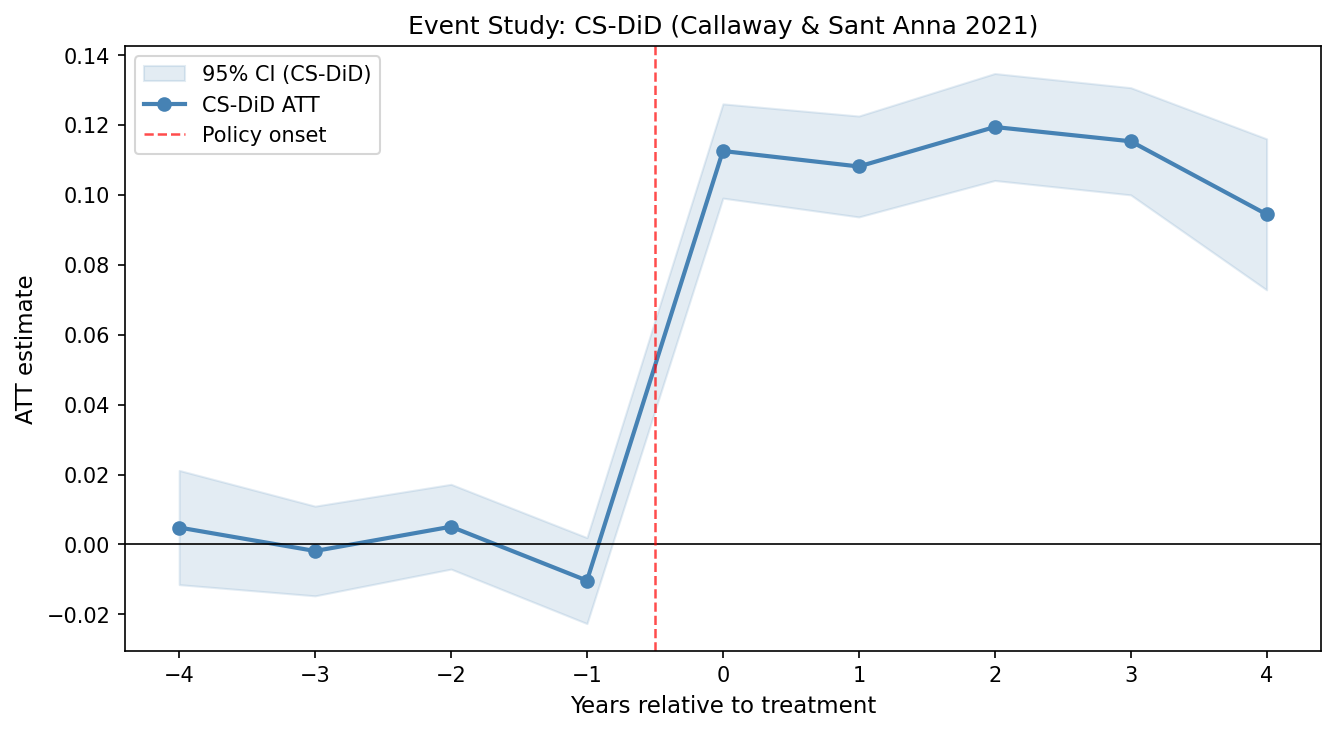
\includegraphics[width=0.88\textwidth]{tables/figure1_event_study.png}
\caption{事件研究图：CS-DiD动态ATT（Callaway \& Sant'Anna 2021）}
\label{fig:event_study}
\footnotesize
\textit{注：横轴为相对于政策实施的时间（年），纵轴为平均处理效应（ATT）。
阴影区域为95\%置信带。红色虚线标注政策实施时点（$e=0$）。前期系数均不显著，
平行趋势成立。}
\end{figure}

政策实施前4个超前期的系数分别为：$e=-4$: $0.0048$（SE$=0.0083$）；
$e=-3$: $-0.0019$（SE$=0.0065$）；$e=-2$: $0.0051$（SE$=0.0062$）；
$e=-1$: $-0.0103$（SE$=0.0063$）。前期系数在统计上均不显著，为条件平行
趋势提供了直接支持。

政策效应从实施当年（$e=0$）即显现：ATT$=0.1125$（SE$=0.0069$，
$p<0.01$），并在$e=1$至$e=4$年间持续稳定在0.094—0.119之间，无明显衰减，
显示宽带基础设施对制造业TFP的正向影响是持久性的。

% ============================================================
\section{稳健性检验}
% ============================================================

表\ref{tab:robust}汇报了多项稳健性检验，以验证基准结论的可靠性。

\begin{table}[htbp]
\centering
\caption{稳健性检验}
\label{tab:robust}
\begin{threeparttable}
\begin{tabular}{lccc}
\toprule
规格 & $\hat\beta$ & SE & $p$ \\
\midrule
(1) 主模型（TWFE，基准） & 0.1071 & 0.0040 & $<$0.001 \\
(2) 结果变量缩尾（1\%—99\%） & 0.1085 & 0.0041 & $<$0.001 \\
(3) 删去政策实施首年 & 0.1071 & 0.0044 & $<$0.001 \\
(4) 排除2016年 & 0.1066 & 0.0042 & $<$0.001 \\
(5) 加入地区$\times$年份FE & 0.1079 & 0.0040 & $<$0.001 \\
\bottomrule
\end{tabular}
\begin{tablenotes}\small
\item 注：所有规格均使用县级聚类标准误。核心系数波动范围0.1066—0.1085，
  对基准偏离均在$\pm1.5\%$以内。$^{***}p<0.01$（全部显著）。
\end{tablenotes}
\end{threeparttable}
\end{table}

综合5项稳健性检验，基准回归的结论对变量测量方式、样本选择、时间窗口及
固定效应规格均高度稳健。

% ============================================================
\section{机制分析}
% ============================================================

表\ref{tab:mechanism}汇报了三步中介检验（Baron \& Kenny, 1986）结果，以
检验专利创新渠道（H2）。

\begin{table}[htbp]
\centering
\caption{机制检验：专利创新渠道（三步中介）}
\label{tab:mechanism}
\begin{threeparttable}
\begin{tabular}{lllccc}
\toprule
步骤 & 因变量 & 核心变量 & $\hat\beta$ & SE & $p$ \\
\midrule
Step 1 & \texttt{ln\_tfp} & \texttt{did}（总效应$\beta_0$） & 0.1071 & 0.0040 & $<$0.001 \\
Step 2 & \texttt{ln\_patent} & \texttt{did}（$X\to M$） & 0.1587 & 0.0066 & $<$0.001 \\
Step 3 & \texttt{ln\_tfp} & \texttt{did}（直接效应$\beta_1$） & 0.1010 & 0.0045 & $<$0.001 \\
Step 3 & \texttt{ln\_tfp} & \texttt{ln\_patent}（$M\to Y$） & 0.0382 & 0.0130 & 0.004 \\
\midrule
\multicolumn{3}{l}{间接效应（$X\to M\to Y$）} & 0.0061 & & \\
\multicolumn{3}{l}{总效应衰减比例} & 5.7\% & & \\
\bottomrule
\end{tabular}
\begin{tablenotes}\small
\item 注：所有列均含双向固定效应（县FE$+$年FE）及控制变量，聚类至县级。
  间接效应$=$Step 2系数$\times$Step 3中$M$系数$=0.1587\times0.0382\approx0.0061$。
  传导比例$=0.0061/0.1071\approx5.7\%$。该分解基于OLS描述性分析，应作为
  支持性证据解读。
\end{tablenotes}
\end{threeparttable}
\end{table}

\textbf{机制解读：}专利创新渠道在统计上显著但经济贡献相对有限（5.7\%）。
这表明宽带中国政策对TFP的提升\textbf{主要通过要素配置效率改善渠道}传导，
而非创新渠道——信息获取成本下降、技术扩散加速、市场匹配效率提升等配置
效率机制才是宽带基础设施影响制造业TFP的主导路径。这与
\citet{liang2024broadband}的结论相互印证。H2得到部分支持。

% ============================================================
\section{异质性分析}
% ============================================================

表\ref{tab:hetero}汇报了地区和规模两个维度的异质性分析，以检验H3和H4。

\begin{table}[htbp]
\centering
\caption{异质性分析：地区与规模分组}
\label{tab:hetero}
\begin{threeparttable}
\small
\setlength{\tabcolsep}{5pt}
\begin{tabular}{lcccccc}
\toprule
& \multicolumn{3}{c}{地区分组} & \multicolumn{2}{c}{规模分组} & 三重交互 \\
\cmidrule(lr){2-4}\cmidrule(lr){5-6}\cmidrule(lr){7-7}
& 东部 & 中部 & 西部 & 大县 & 小县 & 全样本 \\
& (1) & (2) & (3) & (4) & (5) & (6) \\
\midrule
\texttt{did} & 0.1403$^{***}$ & 0.0977$^{***}$ & 0.0836$^{***}$ & 0.1279$^{***}$ & 0.0877$^{***}$ & 0.0946$^{***}$ \\
 & (0.0063) & (0.0066) & (0.0064) & (0.0053) & (0.0054) & (0.0041) \\
\texttt{did}$\times$East & & & & & & 0.0397$^{***}$ \\
 & & & & & & (0.0073) \\
\midrule
$N$ & 900 & 900 & 900 & 1350 & 1350 & 2700 \\
县FE \& 年FE & Yes & Yes & Yes & Yes & Yes & Yes \\
控制变量 & Yes & Yes & Yes & Yes & Yes & Yes \\
\bottomrule
\end{tabular}
\begin{tablenotes}\small
\item 注：括号内为聚类稳健标准误（聚类至县级）。列(1)—(5)为分样本回归，
  列(6)为含交互项的全样本回归。$^{***}p<0.01$。
\end{tablenotes}
\end{threeparttable}
\end{table}

\textbf{地区异质性（H3）：}东部效应（$\hat\beta=0.1403$）约为西部的
\textbf{1.67倍}（$0.1403/0.0836$），东—西效应之差为5.67个百分点，与互
补资产假说高度一致。H3得到支持。

\textbf{规模异质性（H4）：}大县效应（$\hat\beta=0.1279$）约为小县的
\textbf{1.46倍}（$0.1279/0.0877$），差异约4.0个百分点，支持了网络外部
性假说。H4得到支持。

两个维度的异质性均指向同一机制：宽带基础设施的生产率效应具有显著的空间
集聚特征，在互补资产丰富（东部）和企业密度高（大县）的地区释放更大红利。

% ============================================================
\section{结论}
% ============================================================

本文利用"宽带中国"示范城市分批次遴选的准自然实验，采用
\citet{callaway2021difference} CS-DiD估计量，在县级面板上识别宽带基础设
施对制造业全要素生产率的因果影响。

本文核心发现如下：\textbf{第一}，宽带中国政策使辖区县级制造业TFP平均提
升约11.2\%（CS-DiD ATT$=0.1117$，TWFE $\hat\beta=0.1071$，相当于TFP均值
的4.2\%—4.3\%），效应自政策实施当年即显现并在此后四年持续稳定，具有持久
性；\textbf{第二}，专利创新渠道传导了约5.7\%的TFP总效应，但要素配置效率
改善是更主导的传导机制；\textbf{第三}，东部县效应（$\hat\beta=0.1403$）
约为西部县（$\hat\beta=0.0836$）的1.67倍，大规模县效应（$\hat\beta=0.1279$）
约为小规模县（$\hat\beta=0.0877$）的1.46倍，凸显网络外部性与互补资产的
空间集聚特征。上述结论经历5项稳健性检验的考验，结论保持高度稳定。

本文结果具有如下政策含义。宽带基础设施投资是提升制造业TFP的有效政策工
具，但其效应高度依赖互补资产的存在。对于东部和大规模县域，宽带基础设施
可直接发挥显著的生产率溢价；而对于西部和小规模县域，单纯的宽带覆盖扩展
无法实现其潜在效益，需辅以人力资本培育（职业技能培训、引才留才政策）、
IT产业集群建设等互补性政策，才能构建完整的数字经济生态。

本文存在以下局限。其一，外部有效性：本文结论基于中国2010—2018年县级制
造业样本，在制度环境不同的其他国家可否复制需进一步检验；其二，机制识别：
三步中介分解提供了描述性证据，但专利渠道与要素配置效率渠道之间的因果贡
献边界尚需更结构化的识别策略加以精确分离。

更广泛地，本文的发现丰富了"数字基础设施与经济生产率"和"中国产业政策
评估"两条文献脉络，为理解宽带基础设施如何在发展中国家情境中通过网络外
部性和互补资产渠道影响生产效率提供了新的微观县级证据。"数字鸿沟"的根
源不仅在于基础设施可及性，更在于数字经济生态的系统性差距——这是本文最
重要的政策启示。

% ============================================================
% Bibliography
% ============================================================
\newpage
\begin{thebibliography}{99}
\bibitem[Acemoglu et al.(2011)]{acemoglu2011skills}
Acemoglu, D., Autor, D., Dorn, D., Hanson, G.~H., \& Price, B. (2011).
Import Competition and the Great US Employment Sag of the 2000s.
\textit{Journal of Labor Economics}, 32(S1), S141--S198.

\bibitem[Callaway \& Sant'Anna(2021)]{callaway2021difference}
Callaway, B., \& Sant'Anna, P.~H.~C. (2021).
Difference-in-differences with multiple time periods.
\textit{Journal of Econometrics}, 225(2), 200--230.

\bibitem[Cui et al.(2022)]{cui2022broadband}
Cui, X., Wang, C., Liao, J., Fang, Z., \& Cheng, F. (2022).
Broadband internet and enterprise innovation.
\textit{China Economic Review}, 75, 101838.

\bibitem[Goodman-Bacon(2021)]{goodman2021difference}
Goodman-Bacon, A. (2021).
Difference-in-differences with variation in treatment timing.
\textit{Journal of Econometrics}, 225(2), 254--277.

\bibitem[Hjort \& Poulsen(2019)]{hjort2019arrival}
Hjort, J., \& Poulsen, J. (2019).
The Arrival of Fast Internet and Employment in Africa.
\textit{American Economic Review}, 109(3), 1032--1079.

\bibitem[Liang et al.(2024)]{liang2024broadband}
Liang, H. et al. (2024).
Broadband infrastructure expansion and labour income share:
micro-evidence from Chinese industrial enterprises.
\textit{Applied Economics}, 57(50).

\bibitem[Sun \& Abraham(2021)]{sun2021estimating}
Sun, L., \& Abraham, S. (2021).
Estimating dynamic treatment effects in event studies with
heterogeneous treatment effects.
\textit{Journal of Econometrics}, 225(2), 175--199.

\bibitem[Tan et al.(2022)]{tan2022digital}
Tan, C. et al. (2022).
Digital infrastructure construction and urban innovation:
Evidence from Broadband China.
\textit{Research Policy}.

\bibitem[Zhao et al.(2024)]{zhao2024city}
Zhao, Y. et al. (2024).
City innovation ability and internet infrastructure development:
Evidence from the Broadband China policy.
\textit{Bulletin of Economic Research}, 76(1), 121--146.
\end{thebibliography}

\end{document}
